

\begin{figure}[ht]
\centering
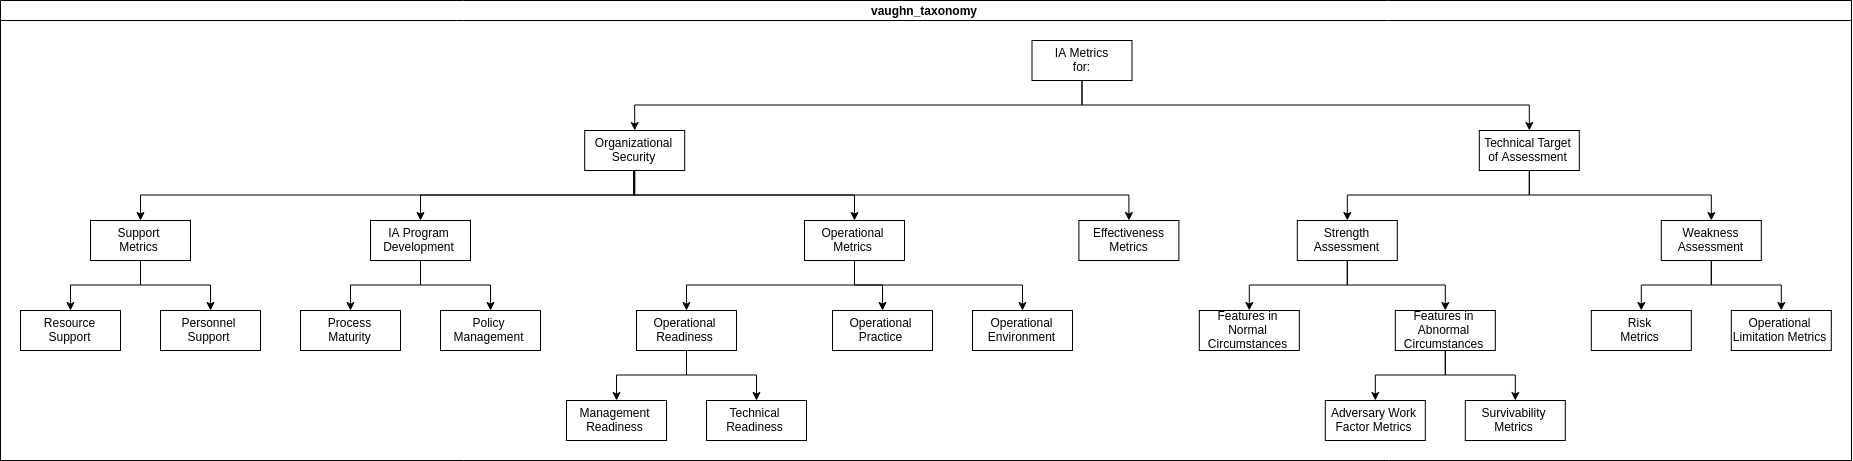
\includegraphics[width=.95\linewidth]{resource/img/ch_background/cybok_metrics/vaughn_taxonomy.png}
\caption{Vaughn's Security Metric Taxonomy\cite{Vaughn_Henning_Siraj_2003}}
\label{fig:background:vaughn_taxonomy}
\end{figure} 

Vaughn’s taxonomy\cite{Vaughn_Henning_Siraj_2003} from 2003 is heavily influenced by federal, and in particular defense department, perspectives on information assurance metrics. The classification tree is heavy on the side of personnel and regulatory metrics compared to other surveys, and the categories draw from military concepts of operational readiness, threat identification, and target acquisition. The survey makes some important observations about properties common to all security metrics. These are presented as binary values which may not be suitable for all metrics, but establishes universal metric attributes we can use in any system.


\begin{figure}[ht]
\centering
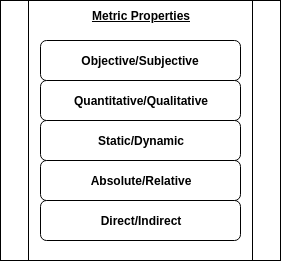
\includegraphics[width=.35\linewidth]{resource/img/ch_background/cybok_metrics/vaughn_metric_propertie.png}
\caption{Vaughn's metric properties\cite{Vaughn_Henning_Siraj_2003}}
\label{fig:background:vaughn_metric_props}
\end{figure} 



\begin{figure}[ht]
\centering
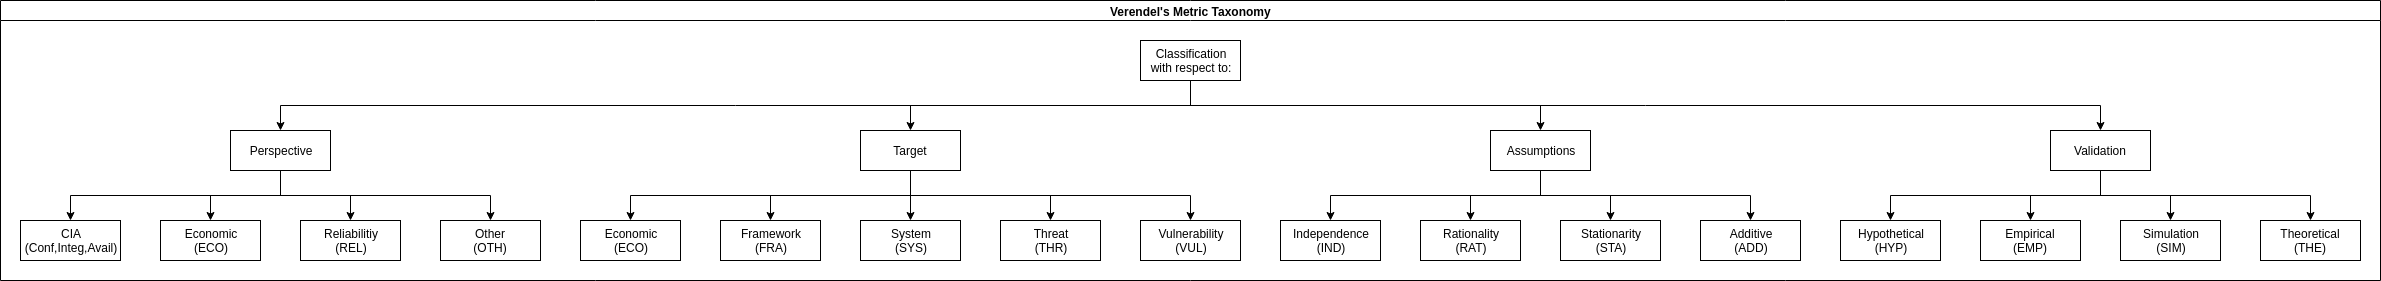
\includegraphics[width=.95\linewidth]{resource/img/ch_background/cybok_metrics/verendel_model_taxonomy.png}
\caption{Verendel's Security Metric Taxonomy \cite{Verendel_2009}}
\label{fig:background:verendel_taxonomy}
\end{figure} 

Verendel’s survey\cite{Verendel_2009} is a critical analysis of the claim that security is quantifiable. The premise is that most of the published models and metrics that attempt to measure security lack the scientific rigor to corroborate or validate their hypothesis. 
The scope of \cite{Verendel_2009} is limited to operational security measurements and assumes measurement primitives include systems, threats, and vulnerabilities.
90 sources published between 1981 and 2008 were surveyed (down selected from 140). These 90 sources are then classified on 4 properties: 
\begin{itemize}
\item \textbf{Perspective}: describes the approach taken to security. { CIA, ECO, REL, OTH}
\item \textbf{Target}: what the source attempts to quantify.{ECO, FRA, SYS, THR, VUL}
\item \textbf{Assumptions}: assumptions made by the source: {IND, RAT, STA, ADD}
\item \textbf{Validation}: how the source supported findings: {HYP, EMP, SIM, THE}
\end{itemize}

Verendel shows that some classes of metrics, specifically cryptographic strength and intrusion detection performance, are validated frequently in the literature through commonly understood methods, while the remaining metric classes are insufficiently validated. 

\begin{figure}[ht]
\centering
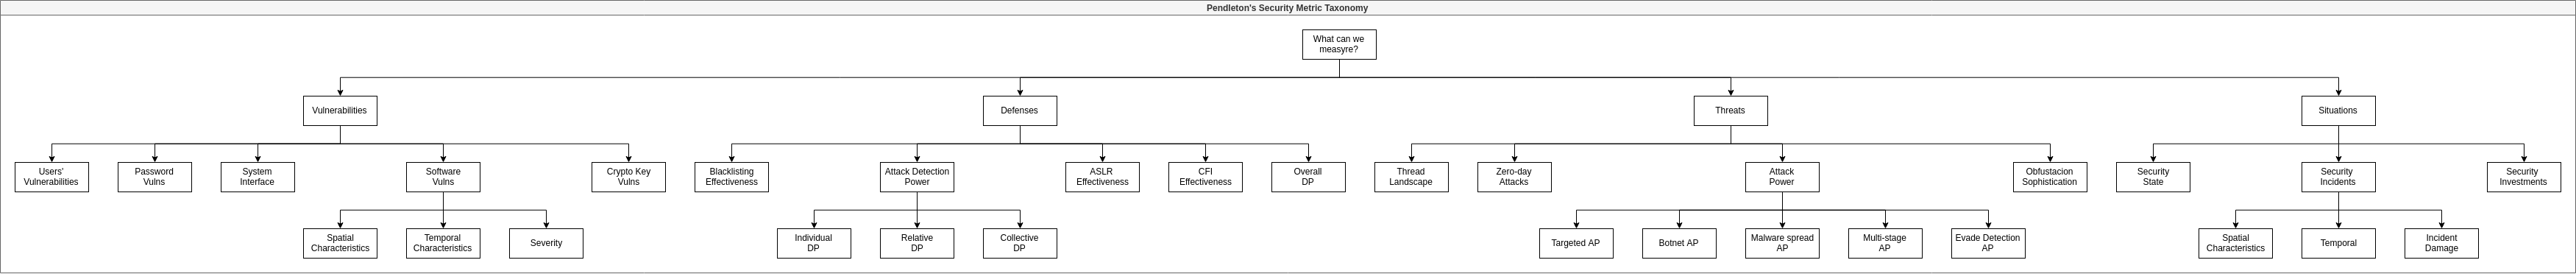
\includegraphics[width=.95\linewidth]{resource/img/ch_background/cybok_metrics/pendleton_metric_taxonomy_drawio.png}
\caption{Pendleton's Security Metric Taxonomy\cite{Pendleton_Garcia-Lebron_Cho_Xu_2016}}
\label{fig:background:pendleton_taxonomy}
\end{figure} 


Pendleton’s survey\cite{ Pendleton_Garcia-Lebron_Xu_2016, Pendleton_Garcia-Lebron_Cho_Xu_2016} approach focuses on metrics that quantify attack and defense interactions. Metrics from 158 sources are classified as measuring one or more of Vulnerabilities, Threats, Defenses, Situations. Situations in this case is a comprehensive metric, with Pendleton’s example subgroups measuring security state over time, successful attacks over time (incident rate), and return on economic investment. Select metrics aligned with Pendleton's survey are shown in Table \ref{tab:pendleton_metrics}.

% \begin{longtable}{@{}llllll@{}}
\begin{tiny}
 \begin{longtable}{@{}|p{0.2\linewidth}|p{0.5\linewidth}|p{0.3\linewidth}|@{}}
% \begin{longtable}{@{}lll@{}}
\toprule
Measuring what? & Representative Metrics Systemized in Paper & Desirable Security Metrics \\* \midrule
\endhead
%
 \multicolumn{3}{c}{\textbf{Measuring System Vulnerabilities}} \\* \midrule
users’ vulnerabilities & user’s susceptibility to phishing attacks \cite{Sheng_Holbrook_Kumaraguru_Cranor_Downs_2010}, user’s susceptibility to malware infection \cite{levesque2013a} & user’s susceptibility to class(es) of attacks (e.g., social-engineering) \\
password vulnerabilities & parameterized/statistical password guessability  \cite{Weir_Aggarwal_Collins_Stern_2010, Bonneau_2012a, Kelley_Komanduri_Mazurek_Shay_Vidas_Bauer_Christin_Cranor_Lopez, Ur_Segreti_Bauer_Christin_Cranor_Komanduri_Kurilova_Mazurek_Melicher_Shay} & worst-case and average-case parameterized\cite{Bonneau_2012b} \\
 &   password entropy\cite{Burr_Dodson_Polk_2006} & password guessability \\
system interface & attack surface \cite{Manadhata_Wing_2010}, exercised attack-surface\cite{Nayak_Marino_Efstathopoulos_Dumitras_2014} & interface-induced susceptibility \\
software vulnerabilities & unpatched vulnerabilities\cite{Chew_Swanson_Stine_Bartol_Brown_Robinson_2008}, exploited vulnerabilities \cite{Nayak_Marino_Efstathopoulos_Dumitras_2014}, vulnerability prevalence \cite{Zhang_Durumeric_Bailey_Liu_Karir_2014} &  \\
vulnerability spatial characteristics &  & vulnerability situation awareness \\
vulnerability temporal characteristics & historical (exploited) vulnerability\cite{Al-Shaer_Khan_Ahmed_2008, Ahmed_Al-Shaer_Khan_2008} , future (exploited) vulnerability \cite{Al-Shaer_Khan_Ahmed_2008, Ahmed_Al-Shaer_Khan_2008}, tendency-to-be-exploited \cite{Sabottke_Suciu_Dumitras}, vulnerability life-time \cite{Frei_Feb_2010, Nappa_Johnson_Bilge_Caballero_Dumitras_2015, Yilek_Rescorla_Shacham_Enright_Savage_2009, durumeric2014a, Zhang_Durumeric_Bailey_Liu_Karir_2014}, & vulnerability vector at any time†, distribution of vulnerability lifetime \\
vulnerability severity & CVSS score {[}of Incident Response and (FIRST) {]}, availability of exploit \cite{Bilge_Dumitras_2012}  & patching priority† , global damage \\
cryptographic key vulnerabilities & vulnerable cryptographic keys \cite{Yilek_Rescorla_Shacham_Enright_Savage_2009, durumeric2014a} Heninger et al. 2012 & (avoidable via prudential engineering) \\* \midrule
 \multicolumn{3}{c}{\textbf{Measuring Defenses} } \\* \midrule
effectiveness of blacklisting & reaction time  \cite{Kuhrer_Rossow_Holz_2014} coverage\cite{Kuhrer_Rossow_Holz_2014}  & blacklisting probability  \\
attack detection power &  &  \\
individual detection power & detection time\cite{Rajab_Monrose_Terzis_2005}, false-positive, false-negative, true-positive, true-negative, ROC, intrusion & detection probability \\
 & detection capability\cite{Gu_Cardenas_Lee_2008}, cost\cite{Gaffney} &  \\
relative detection power & relative effectiveness\cite{Boggs_Stolfo_2011, Boggs_Du_Stolfo_2014} & relative effectiveness against unknown attacks \\
collective detection power & collective effectiveness \cite{Boggs_Stolfo_2011, Morales_Xu_Sandhu_2012, Boggs_Du_Stolfo_2014, Mohaisen_Alrawi_2014, Yardon_2014}& collective effectiveness against unknown attacks \\
ASLR effectiveness & entropy \cite{Shacham_Page_Pfaff_Goh_Modadugu_Boneh_2004}, effective entropy\cite{Herlands_Hobson_Donovan_2014} & security gain†, extra attack effort† \\
CFI effectiveness & CFG accuracy {[}Evans et al. 2015{]}, & CFI resilience† , CFI power  \\
overall defense power & penetration resistance\cite{Levin_2003}, indirect MTD effectiveness\cite{Han_Lu_Xu_2014}& resistance against unknown attacks†, direct MTD effectiveness \\* \midrule
 \multicolumn{3}{c}{\textbf{Measuring Threats}} \\* \midrule
threat landscape & exploit kits {[}Ablon et al. 2014{]}, malicious network\cite{Zhang_Zhang_Ou_2014}, rogue network & comprehensive cyber threat posture \\
 &\cite{Stone-Gross_Kruegel_Almeroth_Moser_Kirda_2009}, ISP badness \cite{Johnson_Chuang_Grossklags_Christin_2012} control-plan reputation\cite{Konte_Perdisci_Feamster_2015}, early-detection time\cite{Konte_Perdisci_Feamster_2015}, cybersecurity posture\cite{Zhan_Xu_Xu_2015}, sweep-time\cite{Zhan_Xu_Xu_2015}, attackrate \cite{Zhan_Xu_Xu_2015} &  \\
zero-day attacks & number of zero-day attacks {[}Corporation 2012{]}, lifetime of zero-day attacks\cite{Bilge_Dumitras_2012}, number of zero-day attack victims \cite{Bilge_Dumitras_2012}& susceptibility of a computer to zero-day attacks \\
attack power &  &  \\
power of targeted attacks & targeted threat index\cite{Hardy_Crete-Nishihata_Kleemola_Senft_Sonne_Wiseman_Gill_Deibert_2014} & susceptibility to targeted attacks \\
power of botnet & botnet size\cite{Dagon_Zou_Lee_2006}, botnet efficiency\cite{Dagon_Gu_Lee_Lee_2007}, botnet robustness\cite{Dagon_Gu_Lee_Lee_2007} & botnet attack power, botnet resilience with counter-countermeasures \\
power of malware spreading & infection rate\cite{Chen_Ji_2007} & attack power , wasted scans \\
power of multi-stage attacks & necessary defense\cite{Sheyner_Haines_Jha_Lippmann_Wing_2002}, weakest adversary\cite{Pamula_Jajodia_Ammann_Swarup_2006}, attack paths & multi-stage attack power \\
 & \cite{Ritchey_Ammann_2000,  Sheyner_Haines_Jha_Lippmann_Wing_2002, Jha_Sheyner_Wing_2002, Cheng_Deng_Li_DeLoach_Singhal_Ou_2014}, k-zero-day-safety &  \\
 & \cite{Wang_Jajodia_Singhal_Noel_2010}, effort-to-security-failure\cite{Dacier_Deswarte_Kaaniche, Ortalo_1999} &  \\
power of evading detection & (no nontrivial metrics defined) & evasion capability \\
obfuscation sophistication & obfuscation prevalence\cite{Roundy_Miller_2013}, packer structural complexity\cite{Ugarte-Pedrero_Balzarotti_Santos_Bringas_2015} & obfuscation sophistication \\* \midrule
 \multicolumn{3}{c}{\textbf{Measuring Situations}} \\* \midrule
security state & fractions of compromised computers at time t, probability a computer is compromised at time t\cite{LeMay_Ford_Keefe_Sanders_Muehrcke_2011, Da_Xu_Xu_2014, Xu_2014a} & S(t) and si (t) for any security incidents   \\
incident spatial characteristics & incident rate \cite{Microsoft_2013, Yen_Heorhiadi_Oprea_Reiter_Juels_2014, levesque2013a}; Maier et al., & incident occurrence frequency \\
 & encounter rate\cite{Yen_Heorhiadi_Oprea_Reiter_Juels_2014,Mezzour_Carley_Carley_2015, Microsoft_2013,levesque2013a} &  \\
incident temporal characteristics & delay in incident detection {[}for Internet Security 2010{]}, time between incidents {[}for Internet Security 2010; & predictive incident occurrence frequency† \\
 & \cite{Jonsson_Olovsson_1997, Madan_Gogeva-Popstojanova_Vaidyanathan_Trivedi_2002, Holm_2014}, time-to-first-compromise &  \\
 & \cite{Jonsson_Olovsson_1997,Madan_Gogeva-Popstojanova_Vaidyanathan_Trivedi_2002,Holm_2014} &  \\
incident damage & cost of incidents {[}for Internet Security 2010{]} & predictive incident damage† \\
security investments & security spending\cite{Chew_Swanson_Stine_Bartol_Brown_Robinson_2008}, security budget {[}for Internet Security 2010{]} & payoff of security investment \\* \bottomrule
\caption{Pendleton's Survey: Selected Attack \& Defense Metrics\cite{Pendleton_Garcia-Lebron_Cho_Xu_2016}}
\label{tab:pendleton_metrics}\\
\end{longtable}
\end{tiny}

In the conclusions Pendleton hints at some properties desirable in all security metrics (additivity) but stops short of declaring these necessary traits for validation, or even enumerating the full list of common metric attributes. 


\begin{figure}[ht]
\centering
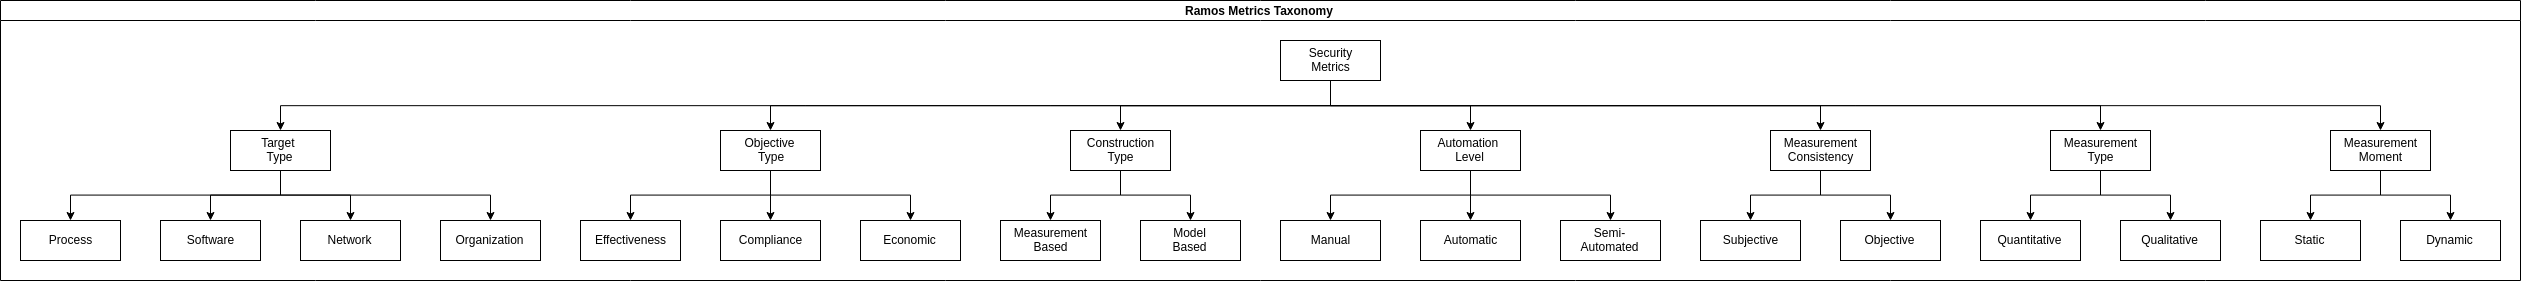
\includegraphics[width=.95\linewidth]{resource/img/ch_background/cybok_metrics/ramos_taxonomy.png}
\caption{Ramos' Security Metric Taxonomy\cite{Ramos_Lazar_Filho_Rodrigues_2017}}
\label{fig:background:ramos_taxonomy}
\end{figure} 

Ramos\cite{Ramos_Lazar_Filho_Rodrigues_2017} focuses on model-based network security metrics exclusively, and provides a list of 5 properties distinct from Vaughn’s in \cite{Vaughn_Henning_Siraj_2003} which all good metrics should possess. Again we see validation listed as necessary to all types of metrics. Ramos cites 146 sources in the survey and consolidates classification to around 75 distinct metrics.

\begin{figure}[ht]
\centering
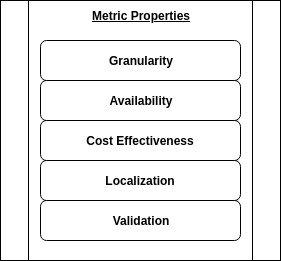
\includegraphics[width=.35\linewidth]{resource/img/ch_background/cybok_metrics/ramos_metric_properties.png}
\caption{Ramos’ Model Based Security Metric Properties\cite{Ramos_Lazar_Filho_Rodrigues_2017}}
\label{fig:background:ramos_metric_props}
\end{figure} 

The primary classification in \cite{Ramos_Lazar_Filho_Rodrigues_2017} is by target. A metric can evaluate a Process (eg SSE-CMM), Software, the Network, or the Organization - which includes physical and personnel security metrics. The Construction Type category distinguishes between empirical and analytical metrics, the latter requiring some type of model (attack graph, markov, etc)  to perform evaluation. Measurement Consistency describes whether a metric is objective or subjective. 

Ramos splits the set of model based quantitative security metrics into 3 buckets based on the input model the metric expects (Stochastic, Graph, Other) with other including attack nets, petri nets, etc. This partitioning is likely to make reporting results easier as, in our experience, these input models will be produced from the same set of input data. Should we consider a metric that computes a function analytically and another that estimates the same quantity through simulation separate metrics? In table IX\cite{Ramos_Lazar_Filho_Rodrigues_2017} Ramos indicates the lack of validation across the surveyed metrics even when the author’s own inline validation we accounted for. Select metrics aligned with Ramos' survey are shown in Table \ref{tab:ramos_metrics}.


\begin{tiny}
\begin{longtable}{@{}lllll@{}}
\toprule
\textbf{Metric} & \textbf{Compliance} & \textbf{Moment} & \textbf{Consistency} &  \\ \midrule
\endhead
%
\bottomrule
\endfoot
%
\endlastfoot
%

MTTF \cite{Dacier_Deswarte_Kaaniche_1996a}\cite{Dacier_Deswarte_Kaaniche} & compliance & dynamic & objective &  \\
METF \cite{Ortalo_1999} & compliance & dynamic & subjective &  \\
MTSF \cite{Almasizadeh_Azgomi_2013a}, \cite{Almasizadeh_Azgomi_2009}, \cite{Almasizadeh_2009} & compliance & static & subjective &  \\
MTFF \cite{Al-Kuwaiti_Kyriakopoulos_Hussein_2009}, \cite{Sallhammar_2006} & compliance & static & subjective &  \\
MTTC by McQueen et al. \cite{McQueen_Boyer_Flynn_Beitel_2005} & compliance & static & subjective &  \\
MTTC by Leversage et al. \cite{Leversage_Byres_2008} & compliance & static & subjective &  \\
Steady-State Security \cite{Almasizadeh_Azgomi_2013a}, \cite{Almasizadeh_Azgomi_2009}, \cite{Almasizadeh_2009} & non-compliance & static & subjective &  \\
Reliability \cite{Jha_Sheyner_Wing_2002} & compliance & static & objective &  \\
Success Likelihood \cite{Kanoun_Dubus_Papillon_Cuppens_Boulahia_Cuppens_2012} & non-compliance & dynamic & subjective &  \\
q \cite{Li_Parker_Xu_2011} & non-compliance & static & objective &  \\
Shortest Path \cite{Phillips_Swiler_1998}, \cite{Idika_Bhargava_2012} & compliance & dynamic & objective &  \\
Number of Paths \cite{Ortalo_1999}, \cite{Idika_Bhargava_2012} & non-compliance & dynamic & objective &  \\
Mean of Path Lengths \cite{Li_Vaughn_2006}, \cite{Idika_Bhargava_2012} & compliance & dynamic & objective &  \\
Normalized Mean of Path Lengths\cite{Idika_Bhargava_2012} & compliance & dynamic & objective &  \\
Assistive metrics: SDPL, MoPL, MePL \cite{Idika_Bhargava_2012} & compliance & dynamic & objective &  \\
Weakest Adversary \cite{Pamula_Jajodia_Ammann_Swarup_2006} & compliance & static &  subjective & \\
Network Compromise Percentage \cite{Lippmann_2006} &  non-compliance &  dynamic &  objective &  \\
Network Compromise Percentage \cite{Lippmann_2006} & non-compliance &  dynamic &  objective & \\
State Rank \cite{Mehta_Bartzis_Zhu_Clarke_Wing_2006} & non-compliance & static & subjective &  \\
Cumulative Score \cite{Noel_Jajodia} & non-compliance & static & objective &  \\
AGP \cite{Wang_Islam_Long_Singhal_Jajodia_2008} & non-compliance & static & subjective &  \\
Attack Resistance \cite{Wang_Singhal_Jajodia_2007a} & compliance & static & subjective &  \\
Enhanced Cumulative Score \cite{Homer_Zhang_Ou_Schmidt_Du_Rajagopalan_Singhal_2013} & non-compliance & static & subjective &  \\
Liu and Man’s metric \cite{Liu_Man_2005} & non-compliance & dynamic & subjective &  \\
Frigault and Wang’s metric \cite{Frigault_Wang_2008} & non-compliance & static & subjective &  \\
Frigault and colleagues’ metric \cite{Frigault_Wang_Singhal_Jajodia_2008} & non-compliance & dynamic & subjective &  \\
Poolsappasit and colleagues’ metric \cite{Poolsappasit_Dewri_Ray_2012} & non-compliance & dynamic & subjective &  \\
Xie and colleagues’ metric \cite{Xie_Li_Ou_Liu_Levy_2010} & non-compliance & dynamic & subjective &  \\
Dantu and colleagues’ metric \cite{Dantu_Kolan_Cangussu_2009}, \cite{Dantu_Kolan_2005}, \cite{Dantu_Loper_Kolan_2004} & non-compliance & dynamic & subjective &  \\
Expected Difficulty \cite{Ghosh_Bhattacharya_2012} & compliance & static & subjective &  \\
VEA-bility \cite{Tupper_Zincir-Heywood_2008} & compliance & static & subjective &  \\
k-zero day safety \cite{Wang_Jajodia_Singhal_Cheng_Noel_2014}, \cite{Wang_Jajodia_Singhal_Noel_2010} & compliance & static & subjective &  \\
d2-Diversity (least attacking effort) \cite{Zhang_Wang_Jajodia_Singhal_Albanese_2016}, \cite{Wang_Zhang_Jajodia_Singhal_Albanese_2014} & compliance & static & subjective &  \\
d3-Diversity (avg. attacking effort) \cite{Zhang_Wang_Jajodia_Singhal_Albanese_2016}, \cite{Wang_Zhang_Jajodia_Singhal_Albanese_2014} & non-compliance & static & subjective &  \\
d1-Diversity (\% of distinct resources) \cite{Zhang_Wang_Jajodia_Singhal_Albanese_2016}, \cite{Wang_Zhang_Jajodia_Singhal_Albanese_2014} & compliance & static & subjective &  \\
Seclius \cite{Zonouz_Berthier_Khurana_Sanders_Yardley_2015} & non-compliance & dynamic & objective &  \\
Damage risk \cite{Chatzipoulidis_Michalopoulos_Mavridis_2015} & non-compliance & static & subjective &  \\
Mean Privacy \cite{Almasizadeh_Azgomi_2013a} & non-compliance & static & subjective &  \\
Security Meter \cite{Sahinoglu_2005}, \cite{Sahinoglu_2008} & non-compliance & static & subjective &  \\
Policy Security Score \cite{Abedin_Nessa_Al-Shaer_Khan_2006} & compliance & dynamic & subjective &  \\
Probabilistic Vulnerability Measure \cite{Ahmed_Al-Shaer_Khan_2008} & non-compliance & dynamic & subjective &  \\
Attack Propagation \cite{Ahmed_Al-Shaer_Taibah_Khan_2011} & non-compliance & dynamic & subjective &  \\
ADVISE \cite{LeMay_Ford_Keefe_Sanders_Muehrcke_2011} & compliance & static & subjective &  \\* \bottomrule
\caption{Ramos' Survey: Selected Model Based Security Metrics\cite{Ramos_Lazar_Filho_Rodrigues_2017}}
\label{tab:ramos_metrics}\\
\end{longtable}
\end{tiny}


\begin{figure}[ht]
\centering
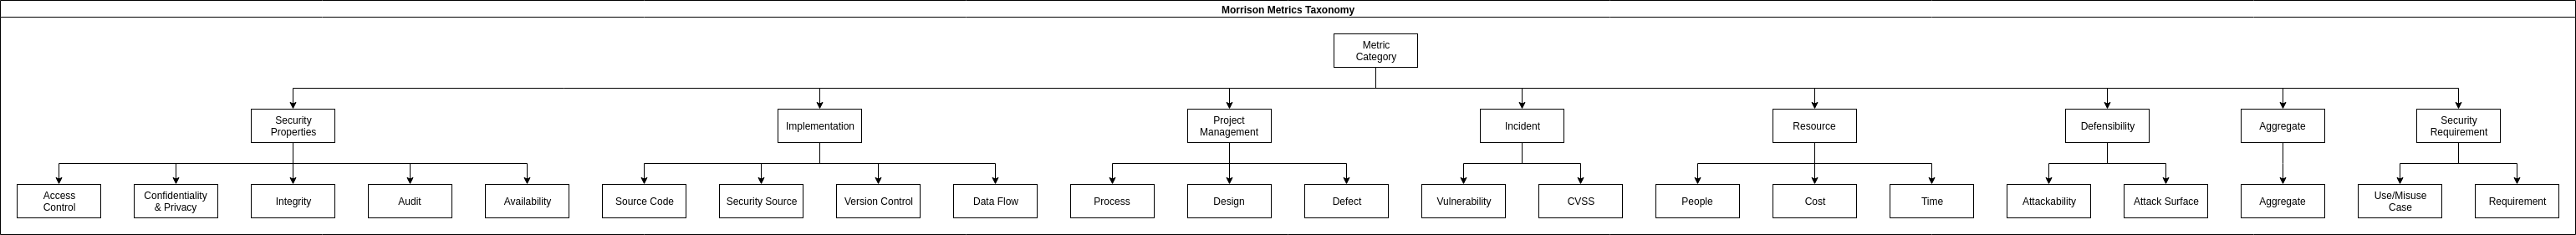
\includegraphics[width=.95\linewidth]{resource/img/ch_background/cybok_metrics/morrison_taxonomy.png}
\caption{Morrison's Security Metric Taxonomy\cite{Morrison_Moye_Pandita_Williams_2018}
\label{fig:background:morrison_taxonomy}}
\end{figure} 

Morrison surveys 71 sources (down selected from 4818) to classify 324 security metrics from the SDLC. The number of metrics for each group are summarized in table \ref{fig:background:morrison_metric_props}.

\begin{tiny}
% \begin{longtable}{@{}llllll@{}}
 \begin{longtable}{@{}p{0.25\linewidth}p{0.15\linewidth}p{0.05\linewidth}p{0.1\linewidth}p{0.1\linewidth}p{0.1\linewidth}@{}}
\cmidrule(r){1-6}
\textit{\textbf{Metric Name}} & \textit{\textbf{Category}} & \textbf{Paper} & \textbf{Method} & \textbf{Scale} & \textbf{Phase} \\* \cmidrule(r){1-6}
\endhead
%
Mechanism strength & Design  & \cite{Liu_Man_2005} & Quantitative & count & Implementation \\
Action Register & Access Control  & \cite{Villarrubia_Fernandez-Medina_Piattini_2006} & Qualitative & count & Operations \\
Alphabet Size & Access Control  & \cite{Villarrubia_Fernandez-Medina_Piattini_2006} & Qualitative & Enumeration & Operations \\
Authentication Period & Access Control  & \cite{Villarrubia_Fernandez-Medina_Piattini_2006} & Qualitative & Enumeration & Operations \\
Block by User Cancellation & Access Control  & \cite{Villarrubia_Fernandez-Medina_Piattini_2006} & Qualitative & ordinal & Operations \\
Group Password & Access Control  & \cite{Villarrubia_Fernandez-Medina_Piattini_2006} & Quantitative & count & Operations \\
Information about Use & Access Control  & \cite{Villarrubia_Fernandez-Medina_Piattini_2006} & Qualitative & Enumeration & Operations \\
Initial Communication & Access Control  & \cite{Villarrubia_Fernandez-Medina_Piattini_2006} & Quantitative & duration & Operations \\
Input Visualization & Access Control  & \cite{Villarrubia_Fernandez-Medina_Piattini_2006} & Qualitative & Enumeration & Operations \\
Maximum Life Time & Access Control  & \cite{Villarrubia_Fernandez-Medina_Piattini_2006} &  & Not specified & Implementation \\
Maximum Number of Erroneous Attempts & Access Control  & \cite{Villarrubia_Fernandez-Medina_Piattini_2006} & Qualitative & ordinal & Operations \\
Minimum Length & Access Control  & \cite{Villarrubia_Fernandez-Medina_Piattini_2006} & Qualitative & ordinal & Operations \\
Minimum Life Time & Access Control  & \cite{Villarrubia_Fernandez-Medina_Piattini_2006} &  & Not specified & Operations \\
Net Transmission & Access Control  & \cite{Villarrubia_Fernandez-Medina_Piattini_2006} & Qualitative & Enumeration & Operations \\
Number of Different Classes & Access Control  & \cite{Villarrubia_Fernandez-Medina_Piattini_2006} &  & Not specified & Operations \\
Password Reassigning & Access Control  & \cite{Villarrubia_Fernandez-Medina_Piattini_2006} & Quantitative & Time & Operations \\
Predefined Users & Access Control  & \cite{Villarrubia_Fernandez-Medina_Piattini_2006} & Qualitative & ordinal & Operations \\
Record Length & Access Control  & \cite{Villarrubia_Fernandez-Medina_Piattini_2006} & Qualitative & ordinal & Operations \\
Selection Restriction & Access Control  & \cite{Villarrubia_Fernandez-Medina_Piattini_2006} & Qualitative & ordinal & Operations \\
Source Selection & Access Control  & \cite{Villarrubia_Fernandez-Medina_Piattini_2006} & Qualitative & ordinal & Operations \\
Storage Class & Confidentiality and Privacy  & \cite{Villarrubia_Fernandez-Medina_Piattini_2006} & Qualitative & Enumeration & Operations \\
User Identificator & Access Control  & \cite{Villarrubia_Fernandez-Medina_Piattini_2006} &  & Not specified & Operations \\
User Training & Access Control  & \cite{Villarrubia_Fernandez-Medina_Piattini_2006} & Quantitative & duration & Operations \\
CVSS Score & CVSS  & \cite{Schryen_Kadura_2009} & Quantitative & count & Operations \\
Patch Index & Vulnerability  & \cite{Schryen_Kadura_2009} & Quantitative & count & Operations \\
Annual Loss Expectancy (ALE) & Cost  & \cite{Bohme_Felegyhazi_2010} & Quantitative & duration & Operations \\
Return on Penetration Testing & Cost  & \cite{Bohme_Felegyhazi_2010} & Qualitative & ordinal & Operations \\
Business Adjusted Risk & Cost  & \cite{Trcek_2010} & Quantitative & count & Operations \\
Daily Vulnerability Exposure & Vulnerability  & \cite{Trcek_2010} & Qualitative & ordinal & Operations \\
Vulnerability Index & Vulnerability  & \cite{Trcek_2010} & Qualitative & ordinal & Operations \\
CN Betweenness & People  & \cite{Meneely_Williams_2010} & Quantitative & count & Operations \\
DN Max Edge Betweenness & People  & \cite{Meneely_Williams_2010} & Quantitative & Time & Operations \\
Num Commits & Version Control  & \cite{Meneely_Williams_2010} & Quantitative & Not specified & Operations \\
NumDevs & People  & \cite{Meneely_Williams_2010} & Qualitative & ordinal & Operations \\
Vulnerability & Vulnerability  & \cite{Meneely_Williams_2010} & Qualitative & ordinal & Operations \\
Contributions & Version Control  & \cite{Perl_Dechand_Smith_Arp_Yamaguchi_Rieck_Fahl_Acar_2015} & Qualitative & ordinal & Operations \\
Fork count & Version Control  & \cite{Perl_Dechand_Smith_Arp_Yamaguchi_Rieck_Fahl_Acar_2015} &  & Not specified & Operations \\
Number of commits & Version Control  & \cite{Perl_Dechand_Smith_Arp_Yamaguchi_Rieck_Fahl_Acar_2015} & Qualitative & ordinal & Operations \\
Number of hunks & Version Control  & \cite{Perl_Dechand_Smith_Arp_Yamaguchi_Rieck_Fahl_Acar_2015} & Qualitative & ordinal & Operations \\
Patch & Version Control  & \cite{Perl_Dechand_Smith_Arp_Yamaguchi_Rieck_Fahl_Acar_2015} & Quantitative &  & Operations \\
Patch keywords & Version Control  & \cite{Perl_Dechand_Smith_Arp_Yamaguchi_Rieck_Fahl_Acar_2015} & Quantitative & count & Operations \\
Programming language & Source Code  & \cite{Perl_Dechand_Smith_Arp_Yamaguchi_Rieck_Fahl_Acar_2015} & Qualitative & currency & Operations \\
Star count & Version Control  & \cite{Perl_Dechand_Smith_Arp_Yamaguchi_Rieck_Fahl_Acar_2015} & Quantitative & ratio & Operations \\
Vulnerability & Vulnerability  & \cite{Perl_Dechand_Smith_Arp_Yamaguchi_Rieck_Fahl_Acar_2015} & Qualitative & currency & Testing \\
Probability Compromised and Repaired (PC) & Attackability & \cite{Marconato_Kaaniche_Nicomette_2013} &  & count & Operations \\
Probability Compromised Not Repaired (PCNR) & Attackability & \cite{Marconato_Kaaniche_Nicomette_2013} & Quantitative & Classes & Design \\
Probability Secure (PS) & Attackability & \cite{Marconato_Kaaniche_Nicomette_2013} & Quantitative & probability & All \\
Probability Unpatched Compromise (PPC) & Attackability & \cite{Marconato_Kaaniche_Nicomette_2013} & Quantitative & ratio & Design \\
Vulnerability Disclosure & Vulnerability  & \cite{Marconato_Kaaniche_Nicomette_2013} &  & probability & Operations \\
Vulnerability Discovery & Vulnerability  & \cite{Marconato_Kaaniche_Nicomette_2013} &  & count & Operations \\
Vulnerability Patch & Vulnerability  & \cite{Marconato_Kaaniche_Nicomette_2013} &  & count & Operations \\
Access Complexity (AC) & CVSS  & \cite{Scarfone_Mell_2008} &  & count & Operations \\
Access Vector (AV) & CVSS  & \cite{Scarfone_Mell_2008} & Quantitative & Classes & Design \\
Authentication (AU) & CVSS  & \cite{Scarfone_Mell_2008} &  & probability & Operations \\
Availability Impact (A) & CVSS  & \cite{Scarfone_Mell_2008} & Quantitative & Ratio & Requirements \\
Availability Requirement (AR) & CVSS  & \cite{Scarfone_Mell_2008} & Quantitative & probability & Operations \\
Collateral Damage Potential (CDP) & CVSS  & \cite{Scarfone_Mell_2008} & Quantitative & probability & Operations \\
Confidentiality Impact (C) & CVSS  & \cite{Scarfone_Mell_2008} & Quantitative & probability & Operations \\
Confidentiality Requirement (CR) & CVSS  & \cite{Scarfone_Mell_2008} & Quantitative & probability & Operations \\
Exploitability (TE) & CVSS  & \cite{Scarfone_Mell_2008} & Quantitative & count & Design \\
Integrity Impact (I) & CVSS  & \cite{Scarfone_Mell_2008} &  & count & Operations \\
Integrity Requirement (IR) & CVSS  & \cite{Scarfone_Mell_2008} & Quantitative & count & Operations \\
Remediation Level (RL) & CVSS  & \cite{Scarfone_Mell_2008} & Quantitative & count & Operations \\
Report Confidence (RC) & CVSS  & \cite{Scarfone_Mell_2008} & Quantitative & count & Operations \\*
\caption{Morrison's Survey: Selected Software Security Metrics\cite{Morrison_Moye_Pandita_Williams_2018}}
\label{tab:morrison_metrics}\\
\end{longtable}
\end{tiny}


\begin{figure}[ht]
\centering
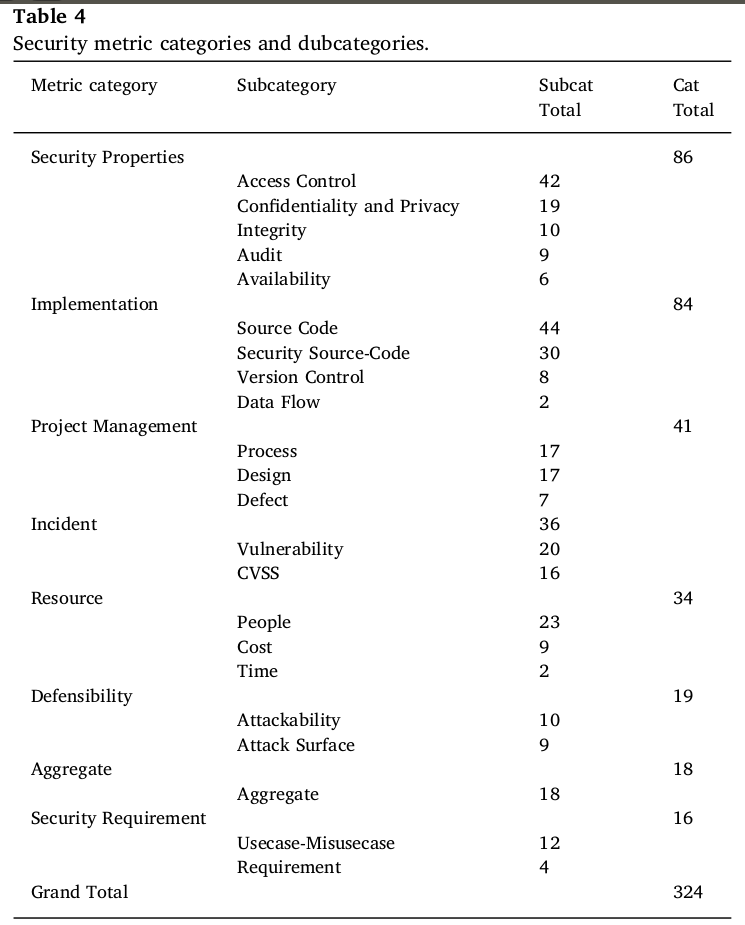
\includegraphics[width=.55\linewidth]{resource/img/ch_background/cybok_metrics/morrison_metric_props_table.png}
\caption{\# Security Metrics by Category/SubCategory (out of 324)\cite{Morrison_Moye_Pandita_Williams_2018}
\label{fig:background:morrison_metric_props}}
\end{figure} 

As these metrics are focused on software security, Morrison finds that many are either normalized to existing software metrics or are extensions thereof. Subcategories of Security Properties seem to be based on surveys about the listed property but this may reflect the source authors rather than an inability to automate collection. Incident Metrics more closely map to previous other’s Vulnerabilities categories as nothing indicates successful attacks are being examined here. 
From the paper’s findings, 85\% of metrics surveyed have only been proposed and evaluated by the author, pointing again to the need for metric validation. Very few metrics apply to design time or test time evaluation in the SDLC - most are tuned for production deployment. The majority of metrics are subjective, relying on user feedback. Select metrics aligned with Morrison's survey are shown in Table \ref{tab:morrison_metrics}.

